\documentclass[12pt]{letter}

\usepackage{amsmath,amssymb}
\usepackage{nopageno}
\usepackage{enumitem}
\usepackage[a4paper, total={7.5in, 11.25in}]{geometry}
\usepackage{tikz}
\usepackage{pgfplots}
\pgfplotsset{compat=1.18}

\usetikzlibrary{calc,3d,decorations.pathmorphing,decorations.pathreplacing,decorations.markings,snakes,arrows.meta,patterns}
\tikzset{snake it/.style={decorate, decoration=snake}}

\begin{document}

Name: \hrulefill \quad Neptun code: \hrulefill

\begin{center}
(KTXFI1EBNF) Physics I. Test~1 \\
May~11,~2026 
\end{center}

\bigskip

\begin{enumerate}
\setcounter{enumi}{0}

\item At what distance from Pluto does a Pluto-stationary satellite orbit in the plane of the equator if it remains constantly above the same point on Pluto's surface? ($M_{\mathrm{Pluto}}=1.305\cdot 10^{22}\,\mathrm{kg}$, \\ $T_{rot}=6.38723\,\mathrm{day}$, $R_{Pluto}=1188\,\mathrm{km}$, $G=6.6743\cdot 10^{-11}\,\mathrm{Nm^2/kg^2}$.)  

\hfill (10~points)

% ------------------------------------------------------------------------------------------------------------------------------------

\bigskip
\item A $5\,\mathrm{kg}$ object slides down a $4$-meter-high incline that makes an angle of $45^\circ$ with the horizontal. What is the speed of the object when it reaches the bottom of the incline if it starts from rest at the top and:
\begin{enumerate}
    \item there is no friction between the object and the incline?
    \item the coefficient of friction is $0.1$? 
    \end{enumerate}
($g=9.81\,\mathrm{m/s^{2}}$) \hfill (10~points)

% ------------------------------------------------------------------------------------------------------------------------------------

\bigskip
\item At a temperature of $30{}^{\circ}\mathrm{C}$, a steel shaft with a diameter of $11.30\,\mathrm{cm}$ needs to be fitted with an aluminum ring with an inner diameter of $11.27\,\mathrm{cm}$ at the same temperature. The linear thermal expansion coefficient of steel is $12 \cdot 10^{-6}\,\mathrm{1/K}$, and the linear thermal expansion coefficient of aluminum is $28.7 \cdot 10^{-6}\,\mathrm{1/K}$. What temperature must the ring be heated to?

\hfill (10~points)

% ------------------------------------------------------------------------------------------------------------------------------------

\bigskip
\item A weather balloon floating at an altitude of several kilometers has a volume of $1800\,\mathrm{m}^{3}$. The temperature and pressure of the helium inside it are the same as those of the surroundings: $-50{}^{\circ}\mathrm{C}$ and $7 \cdot 10^{3}\,\mathrm{Pa}$, respectively.
\begin{enumerate}
\item How many moles of helium are in the balloon?
\item What is the mass of the helium gas? $\left(M = 4\,\frac{\mathrm{g}}{\mathrm{mol}}\right)$
\item What was the volume of the balloon when it was launched from Earth, if the gas inside the balloon was characterized by a temperature of $0{}^{\circ}\mathrm{C}$ and a pressure of $10^{5}\,\mathrm{Pa}$?
\end{enumerate}
($R=8.31\,\mathrm{J/K}$) \hfill (10~points)

% ------------------------------------------------------------------------------------------------------------------------------------

\bigskip
\item An electron enters the region between the parallel plates shown in the figure halfway between the plates. The length of the plates is $l = 12\,\mathrm{cm}$, their separation is $d = 2\,\mathrm{cm}$, and the voltage between them is $U = 300\,\mathrm{V}$. What must the initial velocity of the electron be so that it just exits the region between the plates? 
  
\begin{center}
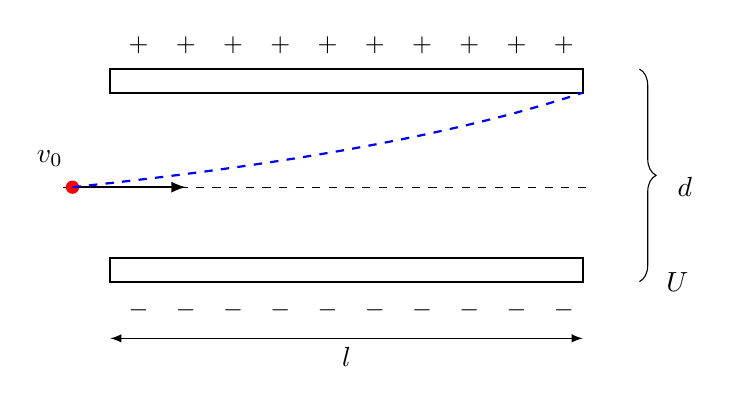
\begin{tikzpicture}[scale=1.2, >=latex]
% Parameters
\def\L{5}    % plate length
\def\d{2}    % plate separation

% Plates
\draw[thick] (0,0) rectangle (\L,0.25);
\draw[thick] (0,-\d) rectangle (\L,-\d+0.25);

% Positive charges: upper plate
\foreach \x in {0.3,0.8,...,4.8}
{
    \node at (\x,+0.5) {\small $+$};
}

% Negative charges: lower plate
\foreach \x in {0.3,0.8,...,4.8}
{
    \node at (\x,-2.3) {\small $-$};
}

% Midline: entry level
\draw[dashed] (-0.5,-\d/2) -- (\L+0.1,-\d/2);

% Electron entry point
\fill[red] (-0.4,-\d/2) circle (2pt);

% Initial velocity
\draw[->, thick] (-0.4,-\d/2) -- (0.8,-\d/2);
\node[left] at (-0.4,-\d/2+0.3) {$v_0$};

% Curved trajectory: just touching the upper plate at the exit
\draw[thick, dashed, blue]
    (-0.4,-\d/2) .. controls (1.5,-\d/2+0.2) and (3.5,-0.5) .. (\L,0.0);

% Length l
\draw[<->] (0,-\d-0.6) -- (\L,-\d-0.6);
\node at (\L/2,-\d-0.8) {$l$};

% Separation d
\draw[decorate, decoration={brace, amplitude=6pt, mirror}]
    (\L+0.6,-\d) -- (\L+0.6,0.25);
\node[right] at (\L+0.9,-\d/2) {$d$};

% Voltage label
\node at (\L+1.0,-\d/2-1.0) {$U$};

\end{tikzpicture}
\end{center}
($m_{e}=9.1\cdot 10^{-31}\,\mathrm{kg}$, $e=1.6\cdot 10^{-19}\,C$) \hfill (10~points)

\end{enumerate}

% ------------------------------------------------------------------------------------------------------------------------------------

Requirement for obtaining the course signature: achieving at least 40\% (20\,points) on the midterm exam.

Grades: 0--25 points: Fail (1), 26--30 points: Pass (2), 31--37 points: Satisfactory (3), 38--45 points:~Good~(4), 46--50 points: Excellent (5).

\rightline{Dr.~Gabor FACSKO}
\rightline{\textit{facsko.gabor@uni-obuda.hu}}

\vfill

\end{document}


